% !TeX root = document.tex
% !TeX encoding = UTF-8 Unicode

\section{Introduction}%
\label{sec:introduction}

\subsection{False Data Injection}%
\label{subsec:fdi}

\begin{slide}{False Data Injection}
  \begin{columns}[c]
    \begin{column}{0.48\textwidth}
      \begin{itemize}
        \item \cmark{}~\textbf{Static False Data Injection}: the attacker
              changes the sensor reading sent, replacing it statically.
        \item \xmark{}~\textbf{Dynamic False Data Injection}: the attacker
              changes the sensor reading dynamically, slowly changing it so
              residuals change slowly.
      \end{itemize}
    \end{column}%
    \hfill%
    \begin{column}{0.48\textwidth}
      \begin{align}
        \tilde{x}_{j} & = x_{i},            \\
        \tilde{x}_{j} & = x_{j}+\delta,     \\
        \tilde{x}_{j} & = x_{j}\cdot\alpha,
      \end{align}
    \end{column}%
  \end{columns}
\end{slide}

\subsection{Functional Observer}%
\label{subsec:functional-observer}

\begin{slide}{Functional Observer}
  \begin{columns}[c]
    \begin{column}{0.48\textwidth}
      \begin{itemize}
        \item \(y(t)\) are the measured outputs.
        \item \(z(t)\) are the states we wish to estimate.
        \item The observer has a reduced order dynamics system which is
              equivalent to the original one.
        \item Problem 1: how to find a \(w(t)\) that correctly estimates
              \(z(t)\).
        \item Problem 2: how to find the observer's matrices \(N,J,H\) and
              \(E\).
      \end{itemize}
    \end{column}%
    \hfill%
    \begin{column}{0.48\textwidth}
      \begin{align}
        \begin{split}
          \dot{x}(t) & = Ax(t) + Bu(t) + Lf(t), \\
          y(t)       & = Cx(t),                 \\
          z(t)       & = Fx(t),
        \end{split} \\\nonumber\\
        \begin{split}
          \dot{w}(t) & = Nw(t) + Jy(t) + Hu(t), \\
          \hat{z}(t) & = w(t) + Ey(t).
        \end{split}
      \end{align}
    \end{column}%
  \end{columns}
\end{slide}

\begin{slide}{Observability}
  \begin{columns}[c]
    \begin{column}{0.48\textwidth}
      \begin{itemize}
        \item All desired states \(z(t)\) must be observable from the outputs
              \(y(t)\).
        \item The observability of \((A,C,F)\) cannot be greater than that of
              \((A,C)\).
        \item There must be a path from every output \(y(t)\) to every output
              \(z(t)\) in the dynamics graph.
      \end{itemize}
    \end{column}%
    \hfill%
    \begin{column}{0.48\textwidth}
      \begin{equation}
        rank
        \begin{bmatrix}
          C \\ CA \\ F \\ FA
        \end{bmatrix}
        = rank
        \begin{bmatrix}
          C \\ CA \\ F
        \end{bmatrix}.
      \end{equation}
    \end{column}%
  \end{columns}
\end{slide}

\begin{slide}{Path Finder Algorithm}
  \begin{figure}[ht!]
    \centering
    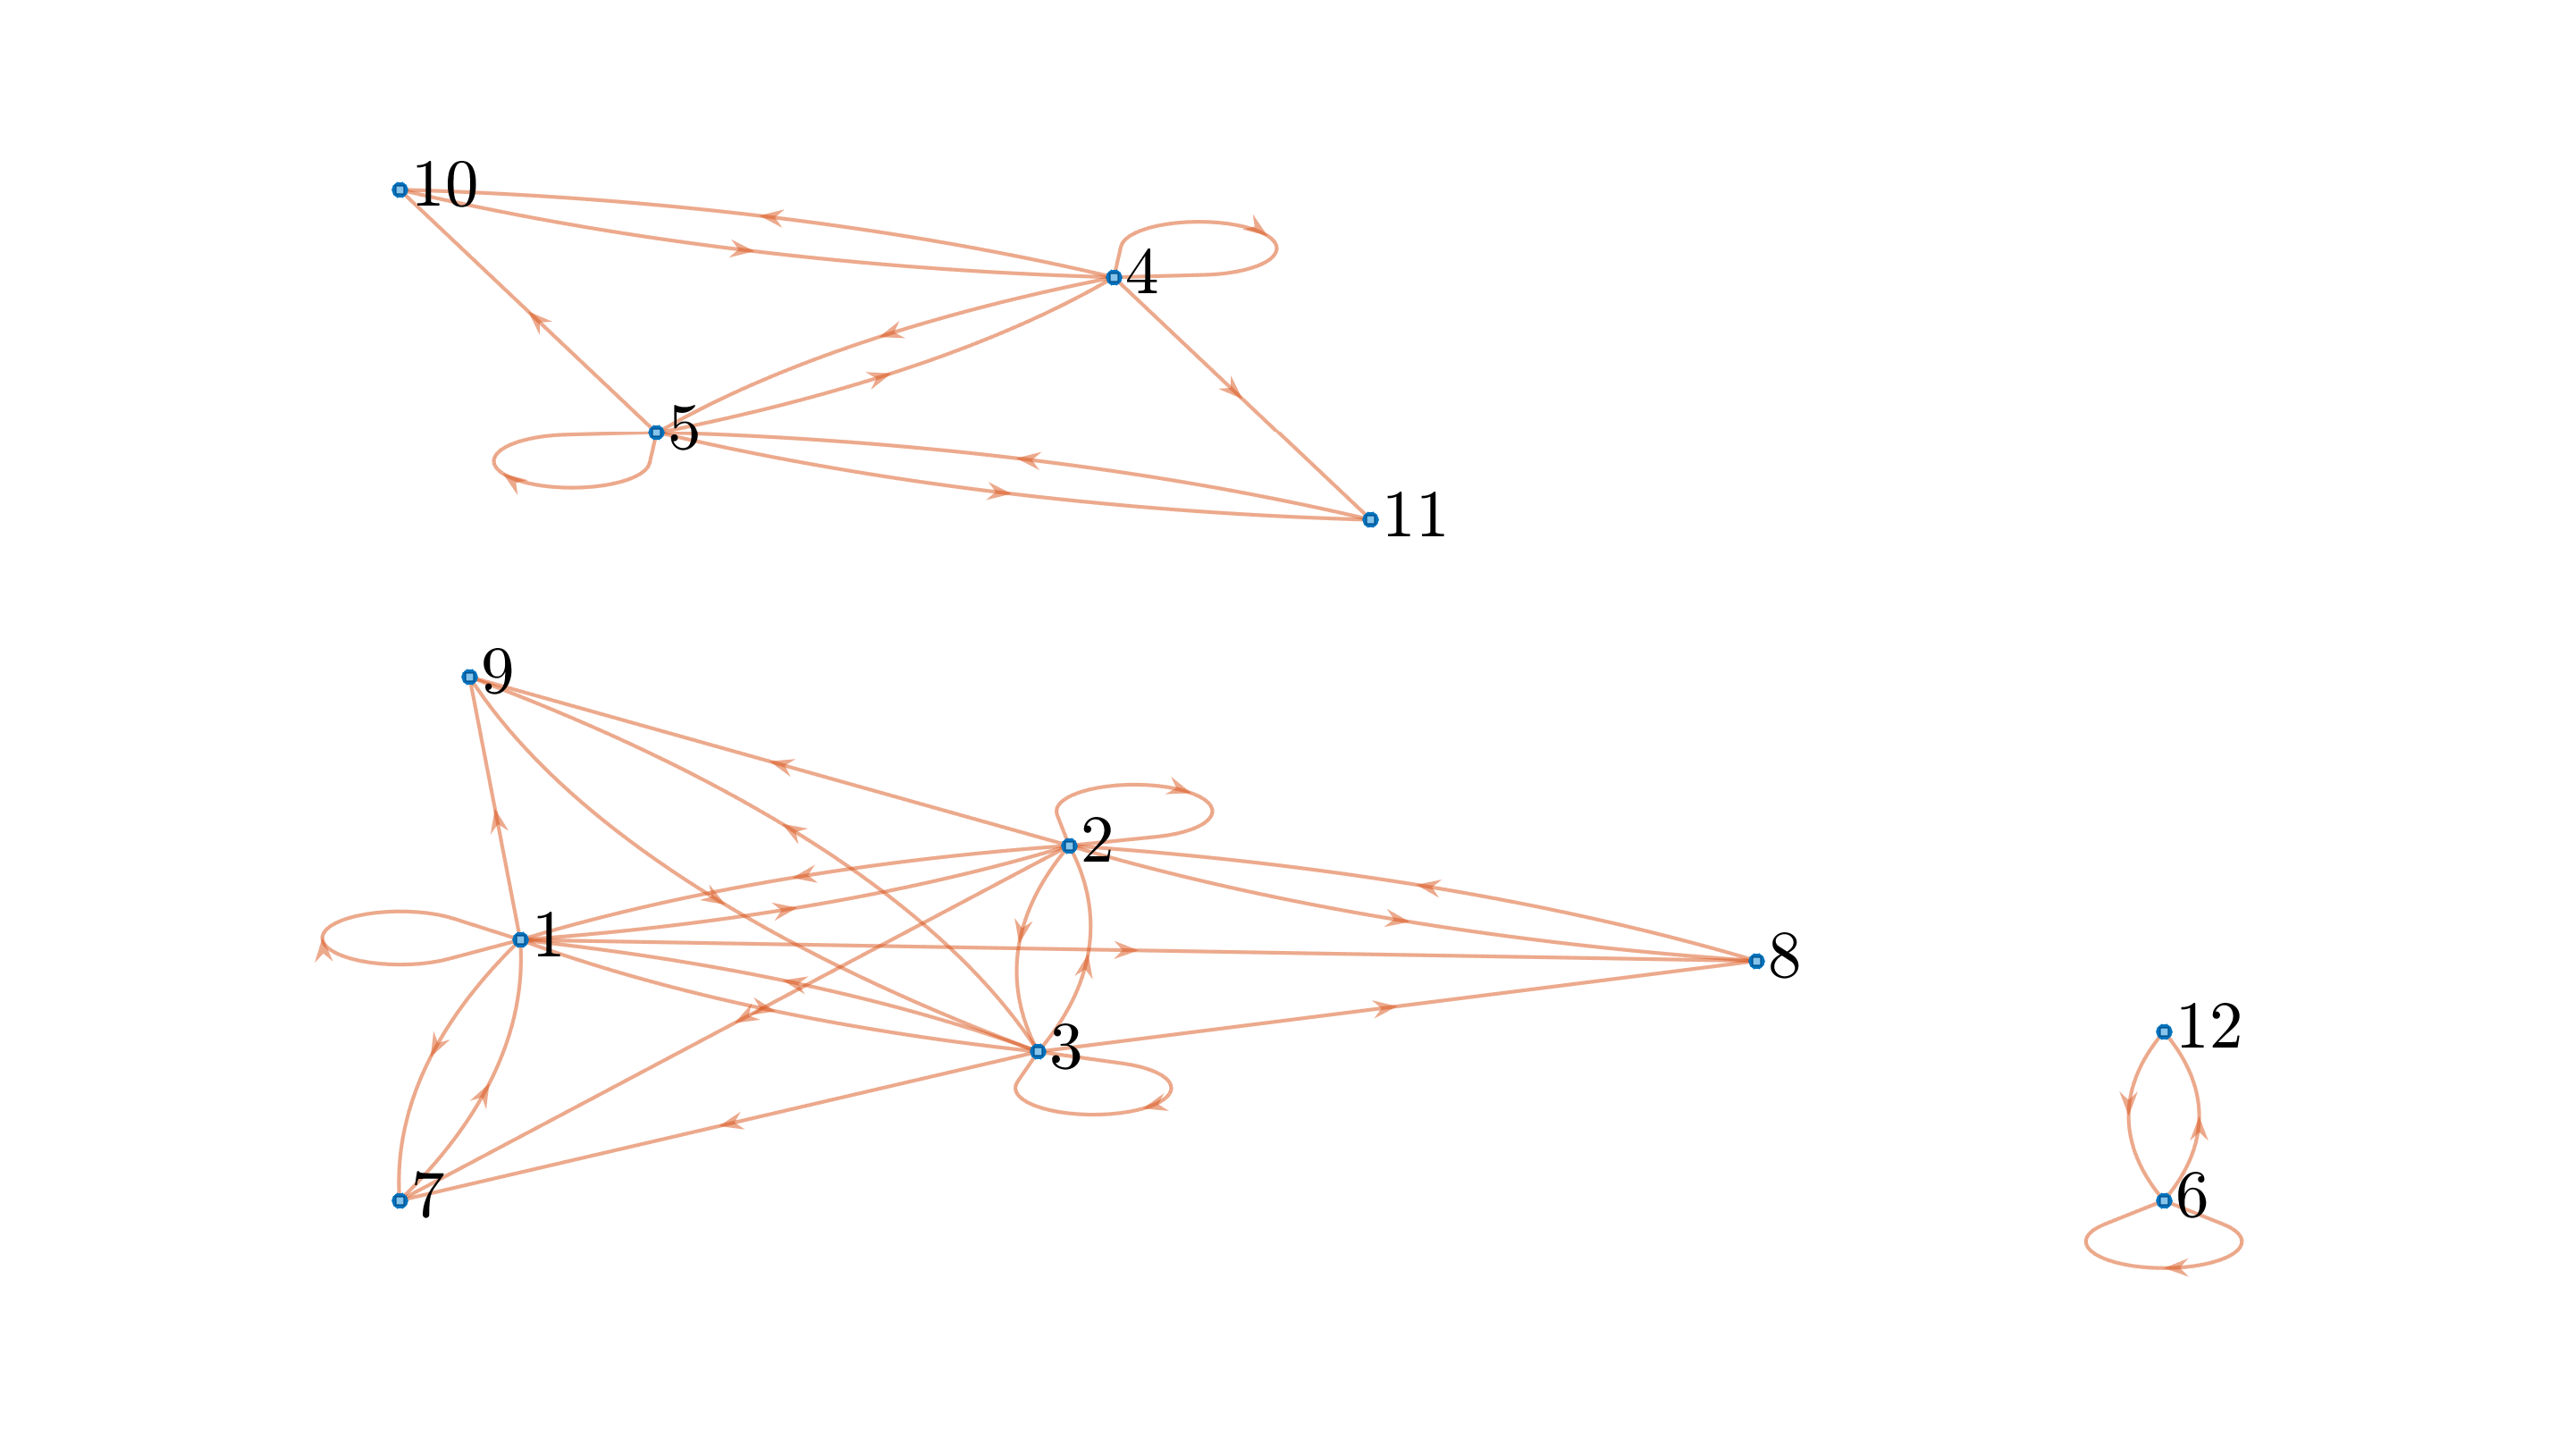
\includegraphics[width=\textheight]{graph-puma}
    \caption{Puma 560 dynamic's graph representation.}%
    \label{fig:puma-graph}
  \end{figure}
\end{slide}
